\documentclass[12pt, french]{article}
\usepackage{circuitikz}
\usepackage{graphicx}
\usepackage{pgfplots}

\usepackage{fancyhdr, fancybox, lastpage, makecell, tikz,}
\usepackage[most]{tcolorbox}
\usepackage[a4paper, margin={0.3in, .75in}]{geometry}
\usepackage{wrapfig}
\pagestyle{fancy}
\renewcommand\headrulewidth{1pt}
\renewcommand\footrulewidth{1pt}
\fancyhf{}
\rhead{ \em{Zakaria Haouzan}}
\lhead[C]{\em{2ème année baccalauréat SM}}
\chead[C]{}
\rfoot[C]{}
\lfoot[R]{ \emph{TD RLC}}
\cfoot[]{\em{Page \thepage / \pageref{LastPage}}}


\newtcolorbox{Box2}[2][
enhanced,
breakable,
]{
                lower separated=false,
                colback=white,
colframe=white!20!black,fonttitle=\bfseries,
colbacktitle=white!30!gray,
coltitle=black,
enhanced,
attach boxed title to top left={yshift=-0.1in,xshift=0.15in},
title=#2,#1}


\begin{document}
\begin{center}
   \shadowbox {\bf{Les oscillations libres dans le circuit RLC }}
\end{center}

\vspace{-0.2cm}
%%_________________________Exercice ! :"_________________________Exercice
%   \begin{center}
	   %\vspace{-0.6cm}
	%\includegraphics[width=0.6\textwidth ]{./img/Exercice01.png}
  %\end{center}



\begin{Box2}{Exercice 1 :Etude du dipôle RC et du circuit LC}
  \section*{}
On réalise le circuit électrique schématisé sur la figure 1. Ce circuit comprend :
\begin{itemize}
    \item Un générateur de f.e.m. $E$, de résistance interne négligeable ;
    \item Une bobine (b) d'inductance $L_0$ et de résistance négligeable ;
    \item Deux conducteurs ohmiques de résistance $r$ et $R = 20\Omega$ ;
    \item Un condensateur de capacité $C$ réglable, initialement déchargé.
\end{itemize}

  \begin{wrapfigure}[23]{r}{0.5\textwidth}
  
    \vspace{-1.5cm}
\begin{center}
  
\begin{circuitikz}[european]
    % Draw the capacitor with voltage label
    \draw (0,-2) coordinate(bot) 
          to[C, l=$C$, v>=$u_c(t)$, *-] (0,2)
          % Add the switch
          node[cute spdt up arrow, rotate=90, anchor=in] (S) {}
          (S.center) node[above=1ex, font=\tiny, scale=0.8] {$t=0$};

    % Draw the resistor R
    \draw (S.out 1) node[above] {pos(1)}
          to[R, l=$R$, v>=$u_R(t)$] ++(-3,0) coordinate (left);

    % Draw the voltage source and resistor r in series
    \draw (left) 
          to[R, l=$r$, v>=$u_r(t)$] ++(0,-2)  
          to[V, invert, l=$E$]  (left|-bot) -- (0,-2);

    % Draw the inductor
    \draw (S.out 2)  -- ++(3,0) coordinate(right)
          to[L, l=$L$, american, v>=$u_L(t)$, *-] (right |- bot) -- (bot);

    % Draw the dashed line for the switch
    \draw [densely dashed] (S.in) -- (S.out 2);

    % Add arrows with labels
    \draw[->, line width=1mm] (0,1.5) -- (2,1.5) node[midway, below] {$Y_A$};
    \draw[->, line width=1mm] (left) -- (-5,4) node[midway, below] {$Y_B$};
\end{circuitikz}


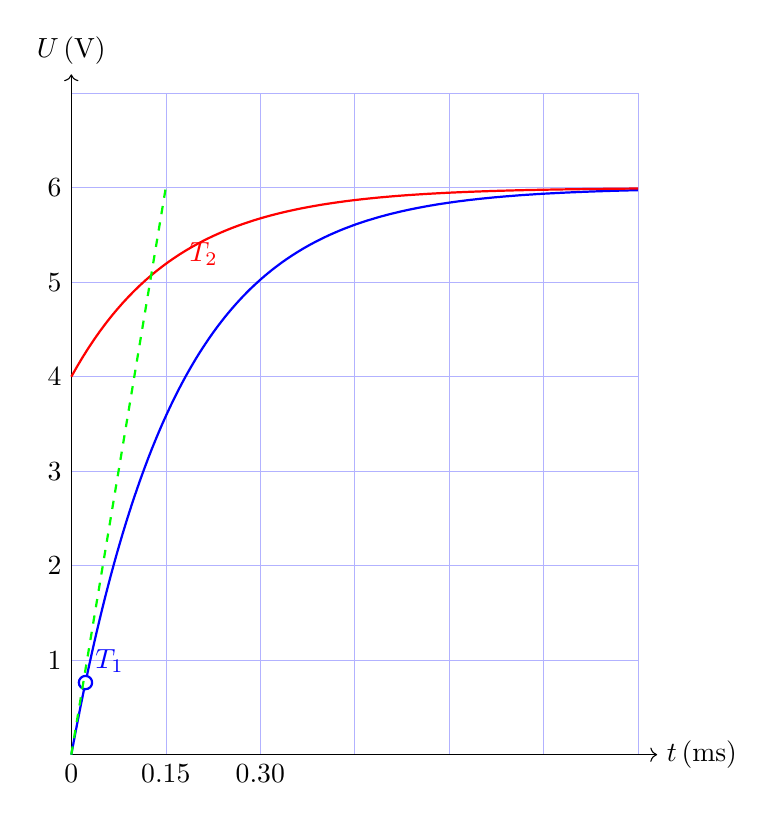
\begin{tikzpicture}[scale=1.2]
    % Grid
    \draw[very thin,color=blue!30] (0,0) grid (6,7);
    
    % Axes
    \draw[->] (0,0) -- (6.2,0) node[right] {$t \, (\text{ms})$};
    \draw[->] (0,0) -- (0,7.2) node[above] {$U \, (\text{V})$};
    
    % Time markers
    \node[below] at (0,0) {$0$};
    \node[below] at (1,0) {$0.15$};
    \node[below] at (2,0) {$0.30$};
    
    % Voltage markers
    \node[left] at (0,1) {$1$};
    \node[left] at (0,2) {$2$};
    \node[left] at (0,3) {$3$};
    \node[left] at (0,4) {$4$};
    \node[left] at (0,5) {$5$};
    \node[left] at (0,6) {$6$};
    
    % Curve T1: U = E(1 - e^(-t/τ))
    \draw[thick, blue] plot[domain=0:6, samples=200] 
        (\x, {6*(1 - exp(-\x/1.1))});
    
    % Hole marking on T1
    \fill[white] (0.15, {6*(1 - exp(-0.15/1.1))}) circle (2pt);
    \draw[thick, blue] (0.15, {6*(1 - exp(-0.15/1.1))}) circle (2pt);
    \node[blue, above right] at (0.15, {6*(1 - exp(-0.15/1.1))}) {$T_1$};
    
    % Curve T2: U = 6 - 3(1 - e^(-t/2))
    \draw[thick, red] plot[domain=0:6, samples=100] 
        (\x, {6 - 2*(exp(-\x/1.1))});
    \node[red] at (1.4,5.3) {$T_2$}; % Label for T2
    
    % Tangent line at t=0 for T1 (slope = E/τ at t=0)
    \draw[thick, dashed, green] (0,0) -- (1, 6) node[above right]{};
    
    
\end{tikzpicture}

\end{center}

\end{wrapfigure}

On fixe la capacité du condensateur sur la valeur $C_0$. À un instant de date $t = 0$, on place l'interrupteur $K$ en position (1). Un système d'acquisition informatisé permet de tracer les courbes $(T1)$ et $(T2)$ de la figure 2 représentant les tensions obtenues en utilisant les voies $Y_1$ et $Y_2$. La droite $(T)$ représente la tangente à la courbe $(T1)$ à $t=0$.

\begin{enumerate}
    \item[1-1] Identifier parmi les courbes $(T1)$ et $(T2)$ celle qui représente la tension $u_c(t)$.
    
    \item[1-2] Établir l'équation différentielle vérifiée par la tension $u_c(t)$.
    
    \item[1-3] Montrer que l'expression de l'intensité du courant juste après avoir placé l'interrupteur en position (1) est $i_0 = \frac{E}{R+r}$
    
    \item[1-4] À l'aide des deux courbes :
    \begin{enumerate}
        \item[1-4-1] Déterminer la valeur de $r$
        \item[1-4-2] Montrer que $C_0 = 5\mu F$
    \end{enumerate}
\end{enumerate}

  \section*{2-Etude du circuit LC idéal}
  Une fois le régime permanent établi, on bascule l’interrupteur $K$ en position (2) à un instant que l’on choisira comme nouvelle origine des dates $(t=0)$. On obtient ainsi un circuit LC.

\begin{enumerate}
    \item Établir l’équation différentielle vérifiée par l’intensité du courant $i(t)$.
    \item La solution de l’équation différentielle s’écrit sous la forme $i(t) = I_m \cos \left( \frac{2\pi}{T_0} t + \varphi \right)$, où $T_0$ représente la période propre de l’oscillateur et $\varphi$ la phase à $t=0$. $I_m$ est l’intensité maximale du courant électrique. Déterminer la valeur de $\varphi$.
    \item Établir, à partir de l’expression de la puissance électrique, l’expression de l’énergie $E_e(t)$ emmagasinée dans le condensateur en fonction de la charge $q(t)$ et de la capacité $C$ du condensateur.
    \item La courbe représentée sur la figure 3 donne l’évolution de l’énergie électrique $E_e(t)$ emmagasinée dans le condensateur en fonction du temps.

      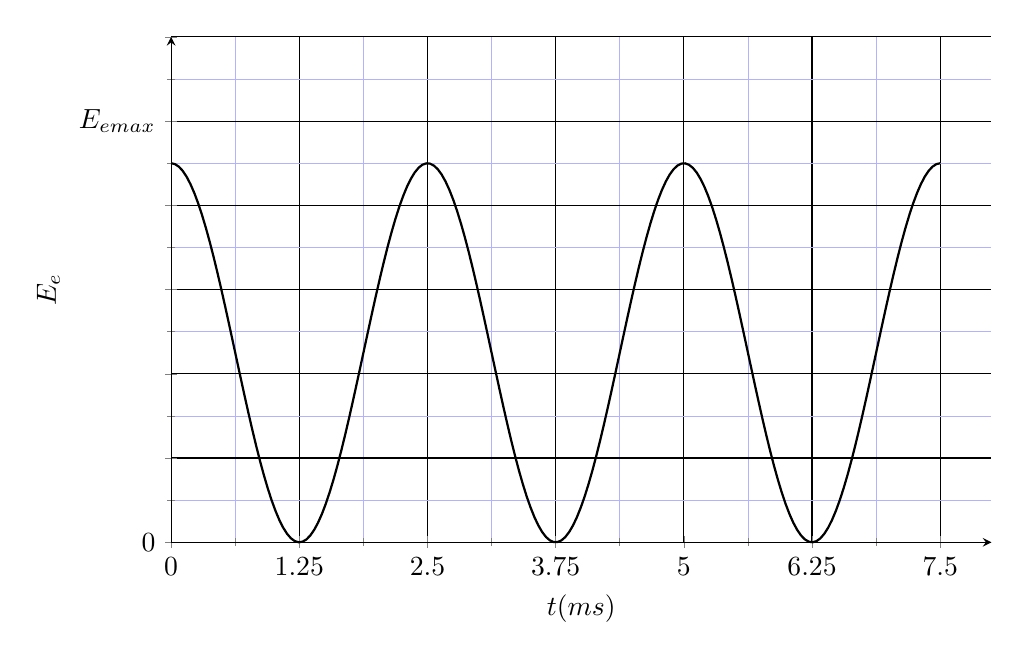
\begin{tikzpicture}
\begin{axis}[
    xlabel={$t(ms)$},
    ylabel={$E_e$},
    xmin=0,
    xmax=8,
    ymin=0,
    ymax=6,
    xtick={0,1.25,2.5,3.75,5,6.25,7.5},
    ytick={0,1,2,3,4,5,6,7},
    yticklabels={0,,,,,$E_{emax}$},
    grid=both,
    minor x tick num=1,  % 4 minor ticks between major ticks
    minor y tick num=1,  % 4 minor ticks between major ticks
    major grid style={black, thin},
    minor grid style={blue!30, very thin},
    width=12cm,
    height=8cm,
    axis lines=left,
    clip=false
]

% Plotting the cos^2 function
\addplot[
    domain=0:7.5,
    samples=200,
    thick,
    black
    ] {4.5 * cos(deg(2*pi*0.2*x))^2};

\end{axis}
\end{tikzpicture}

    \begin{enumerate}
        \item Calculer l’énergie électrique maximale $E_{c\max}$.
        \item À l’aide d’une étude énergétique, trouver la valeur de $I_m$.
    \end{enumerate}
\end{enumerate}
\end{Box2}


\begin{Box2}{Exercice 2 :Etude du circuit LC}


  \emph{Le dipôle LC se comporte comme un oscillateur dans lequel s’effectue périodiquement un échange d’énergie
entre le condensateur et la bobine ; mais ,en réalité ,l’énergie totale de ce dipôle ne reste
pas constante au cours du temps à cause des pertes d’énergie par effet joule .
L’objectif de cet exercice est d’étudier l’échange énergétique entre le condensateur et la bobine ainsi que la
réponse d’une bobine à un échelon de tension électrique .}

  \begin{wrapfigure}[0]{r}{0.3\textwidth}
  \vspace{-0.5cm}
  \begin{center}
    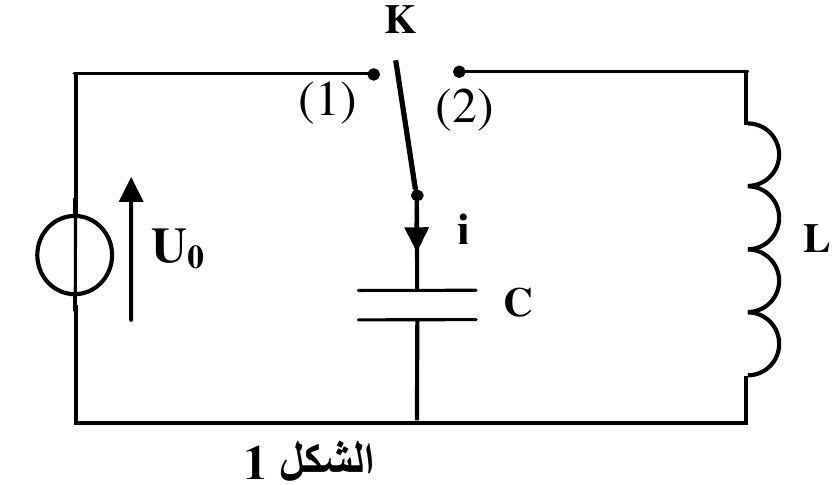
\includegraphics[width=0.3\textwidth]{./img/fig00RLC.png}
  \end{center}
\end{wrapfigure}

\subsubsection*{1- Oscillations électriques dans le cas où la bobine a une résistance négligeable}
On considère le montage de la figure 1 qui comprend :
\begin{itemize}
    \item Un générateur idéal de tension qui donne une tension $U_0$
    \item Une bobine d'inductance L et de résistance négligeable
    \item Un condensateur de capacité $C = 8,0.10^{-9}$ F
    \item Un interrupteur K
\end{itemize}

On charge le condensateur sous la tension $U_0$ en plaçant l'interrupteur dans la position (1).
Lorsque le condensateur est complètement chargé, on bascule l'interrupteur dans la position (2) à l'instant $t = 0$, il passe alors dans le circuit un courant d'intensité i.

A l'aide d'un dispositif approprié, on visualise la courbe représentant les variations de l'intensité i en fonction du temps (figure 2) et la courbe représentant les variations de l'énergie magnétique $E_m$ emmagasinée dans la bobine en fonction du temps (figure 3).
  \begin{center}
    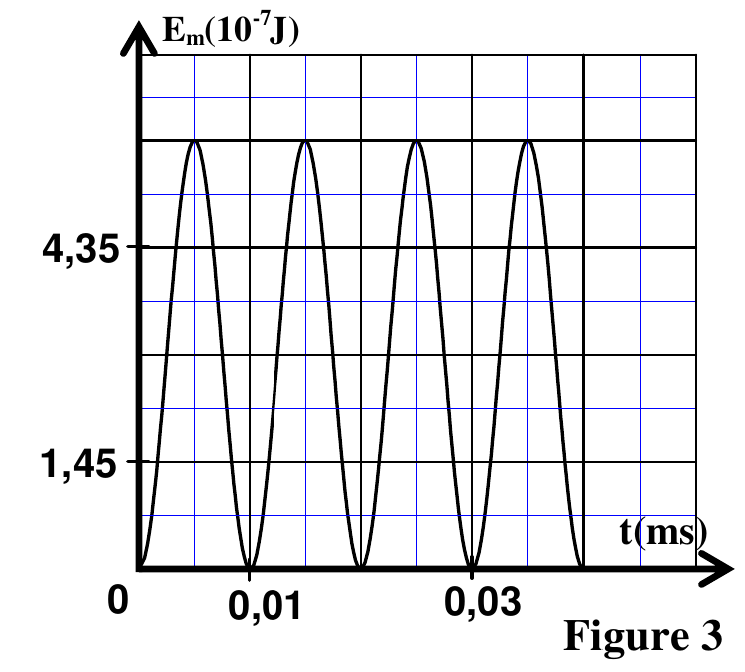
\includegraphics[width=0.3\textwidth]{./img/fig01RLC.png}
    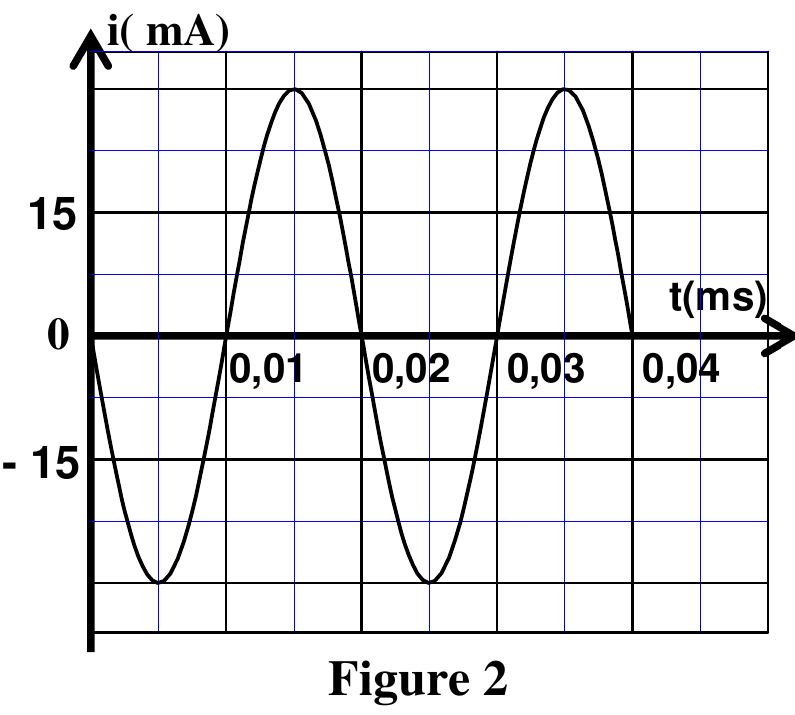
\includegraphics[width=0.3\textwidth]{./img/fig02RLC.png}
  \end{center}


\begin{enumerate}
  
  \item[1.1]  Trouver l'équation différentielle vérifiée par l'intensité i du courant.

  \item[1.2] A l'aide des figures (2) et (3) :
\begin{enumerate}
  \item[a-] Déterminer la valeur de l'énergie totale $E_T$ du circuit LC et en déduire la valeur de $U_0$.
  \item[b-] Déterminer la valeur de L.
\end{enumerate}

\end{enumerate}
\subsubsection*{2- Réponse d'une bobine de résistance négligeable à \\ un échelon de tension}

  \begin{wrapfigure}[4]{r}{0.4\textwidth}
  \vspace{-3.5cm}
  \begin{center}
    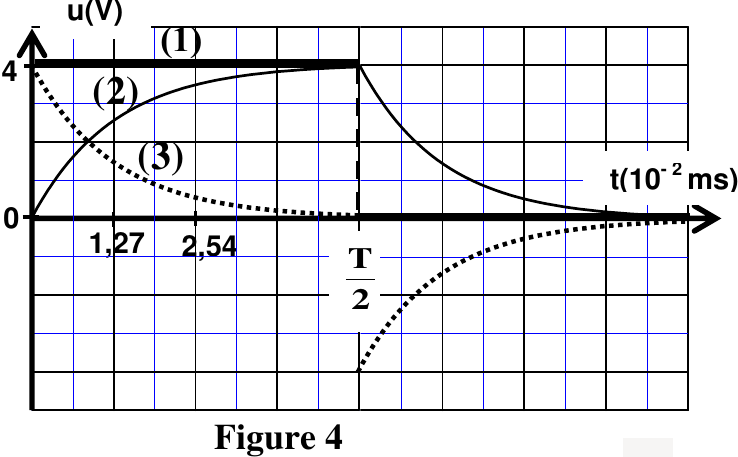
\includegraphics[width=0.4\textwidth]{./img/fig03RLC.png}
  \end{center}
\end{wrapfigure}
On monte la bobine précédente en série avec un conducteur ohmique de résistance $R = 100 \Omega$. On applique entre les bornes du dipôle obtenu un échelon de tension de valeur ascendante E et de valeur descendante nulle et de période T.

On visualise à l'aide d'un dispositif approprié l'évolution de la tension u entre les bornes du générateur, la tension $u_R$ aux bornes du conducteur ohmique et la tension $u_L$ aux bornes de la bobine mon obtient alors les courbes (1), (2) et (3) représentées dans la figure 4.
\begin{enumerate}
  
  \item[2.1] Etablir l'équation différentielle vérifiée par l'intensité du courant i(t) dans l'intervalle $0 \leq t < \frac{T}{2}$.

  \item[2.2] La solution de cette équation différentielle s'écrit sous la forme :
\[ i(t) = I_p(1-e^{-\frac{t}{\tau}}) \]
avec $I_p$ et $\tau$ des constantes.
\begin{enumerate}
  \item[a-] Associer chacune des tensions $u_L$ et $u_R$ à la courbe correspondante dans la figure 4.
  \item[b-] A l'aide des courbes de la figure 4, trouver la valeur de $I_p$.
\end{enumerate}

\item[2.3] L'expression de l'intensité du courant s'écrit dans l'intervalle $\frac{T}{2} \leq t < T$ (sans changer l'origine du temps) sous la forme :
\[ i(t) = A.e^{-\frac{t}{\tau}} \]
avec A et $\tau$ des constantes.

Montrer que l'expression de l'intensité du courant à l'instant $t_1 = \frac{3T}{4}$ s'écrit sous la forme $i(t_1) $=$I_p.e^{-2}$.

\end{enumerate}
\subsubsection*{3- Les oscillations électriques dans le cas où la bobine a une résistance non négligeable}
On répète l'expérience en utilisant le montage représenté dans la figure 1 en remplaçant la bobine précédente par une autre bobine ayant la même inductance L, mais sa résistance r n'est pas négligeable.

Après avoir chargé complètement le condensateur, on bascule l'interrupteur dans la position (2).
La figure 5 représente l'évolution de la charge q du condensateur en fonction du temps.

  \begin{center}
    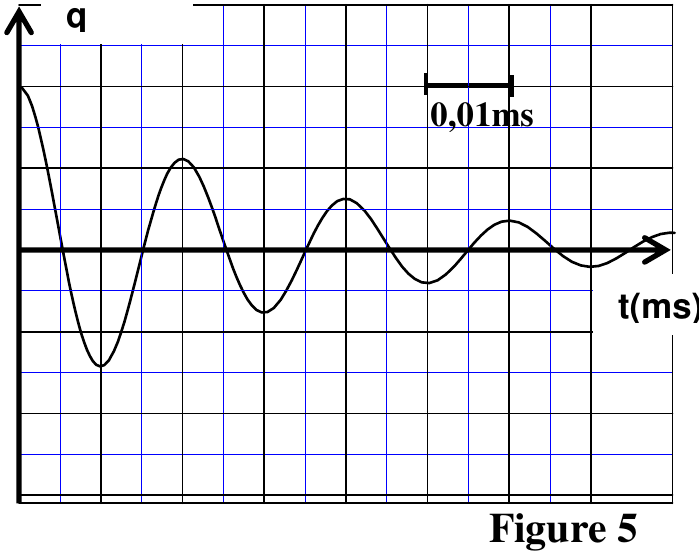
\includegraphics[width=0.4\textwidth]{./img/fig04RLC.png}
  \end{center}

\begin{enumerate}
  
  \item[3.1] Choisir la ou les réponses justes :
L'énergie emmagasinée dans la bobine est :
\begin{enumerate}
  \item[a-] maximale à l'instant $t_1 = 5.10^{-3}$ ms
  \item[b-] minimale à l'instant $t_1 = 5.10^{-3}$ ms
  \item[c-] maximale à l'instant $t_2 = 10^{-2}$ ms
  \item[d-] minimale à l'instant $t_2 = 10^{-2}$ ms
\end{enumerate}

\item[3.2] Montrer que l'équation différentielle vérifiée par la charge du condensateur s'écrit sous la forme :
\[ \frac{d^2q}{dt^2} + 2\lambda\frac{dq}{dt} + \frac{4\pi^2}{T_0^2}q = 0 \]
avec $T_0$ la période propre du circuit et $\lambda = \frac{r}{2L}$.

\item[3.3] Sachant que l'expression de la pseudo période T des oscillations est :
  \[ T = \frac{1}{\sqrt{\frac{1}{T_0^2}-\frac{\lambda^2}{4\pi^2}}} \]
trouver la condition que doit vérifier r par rapport à $\sqrt{\frac{L}{C}}$ pour que $T \approx  T_0$.

\end{enumerate}
\end{Box2}
%%_________________________Exercice !2 :"_________________________Exercice
\end{document}
